\section{Aufbau}
In dem beschriebenen Experiment wurde ein Aufbau der Firma Helmut Fischer GmbH verwendet wie in Abbildung \ref{fig:Aufbau} zusehen ist.\\
Als Energiequelle zur Anregung der Elektronen wird eine Röntgenröhre verwendet, mit einer Beschleunigungsspannung von 30-50kV. In dem durchgeführten Versuch wurde zur Materialanalyse eine Beschleunigungsspannung von 50 kV verwendet. Wodurch sich eine maximale Photonenenergie des Kontinuierlichen Spektrums von 50keV ergibt. \\
Das so entstandene kontinuierliche Spektrum kann durch verschiedene Filter, die in den Strahlengang eingebracht werden können, verändert werden. Die Filter befinden sich in der Abbildung \ref{fig:Aufbau} unterhalb der Röntgenröhre.\\
Trifft die Strahlung auf die Probe, wird ein großer Teil absorbiert.\\
Die entstehende Fluoreszenzstrahlung kann mit Hilfe eines Siliziumdriftdetektors gemessen und analysiert werden.
Zudem ist eine Kamera installiert worden mit der die Probe ausgerichtet werden kann, jedoch hat sie keinen Einfluss auf die Messungen sondern dient lediglich der Justage.\\
\begin{figure}[h]
 \centering
 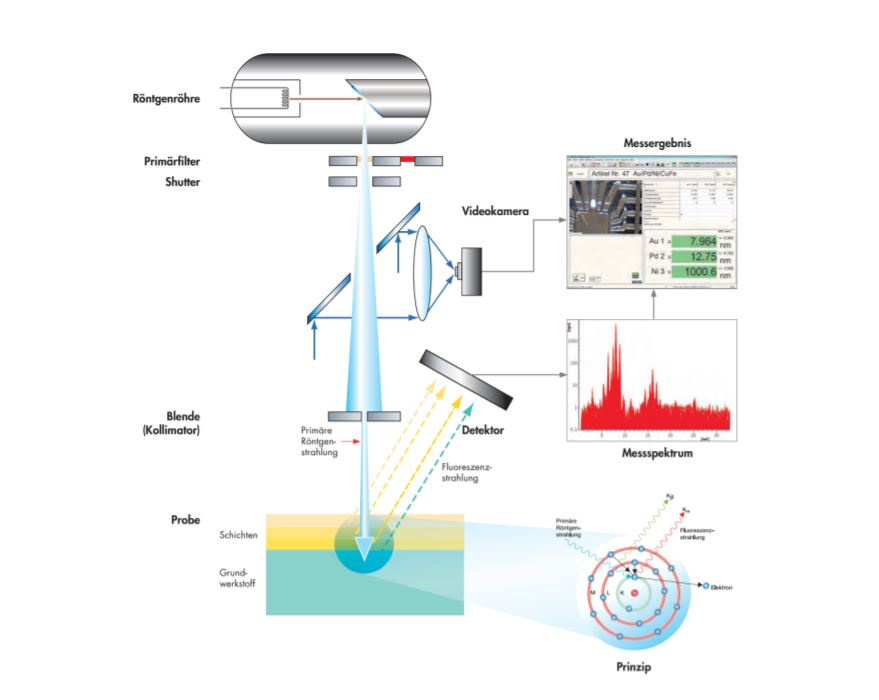
\includegraphics{XRF.JPG}
 \caption[Fischer XRF]{Aufbau des Fischer Röntgen-Fluoreszenzspektrometer \cite{bib:Aufbau}}
 \label{fig:Aufbau}
\end{figure}
[filter in diesen teil]